\section{Node Distance and Embedding Distance}

We examine whether statements that are closer in the dependency graph also
have more similar slogan embeddings. Specifically, we measure the cosine
similarity between pairs of statements separated by a directed graph distance of $d$ dependency edges. Figure~\ref{fig:cos-dist} reports results for parent-only trajectories.

\subsection{Setup}

For each formality and depth $d$, we collected 1,000
accepted statement pairs. Starting from a randomly sampled initial statement seed, we repeatedly sampled one parent/dependency uniformly at random. At depth $d$, we retained the resulting pair only when its directed shortest-path distance from the seed was exactly $d$. Thus, accepted walks contain no directed shortcut of length less than $d$.

Each depth was sampled independently. In particular, failed walks were
replaced, and a new initial seed redrawn, until reaching the target number of accepted observations, so the
samples at depth $d$ should not be interpreted as continuations of the same
trajectories used at depth $d-1$.

For embedding comparison, we used sloganized statements embedded with
Qwen3-8B. Embeddings are $\ell_2$-normalized before cosine similarity is
computed as their dot product. Error bars show pointwise 95\%
normal-approximation confidence intervals for the mean cosine similarity.
The dashed horizontal line denotes a graph-free random-pair baseline,
computed separately for the formal and informal corpora as the mean cosine
similarity over 1,000 randomly paired, distinct statements.

\subsection{Results}

\begin{figure}[h]
    \centering
    
    \begin{subfigure}{0.48\textwidth}
        \centering
        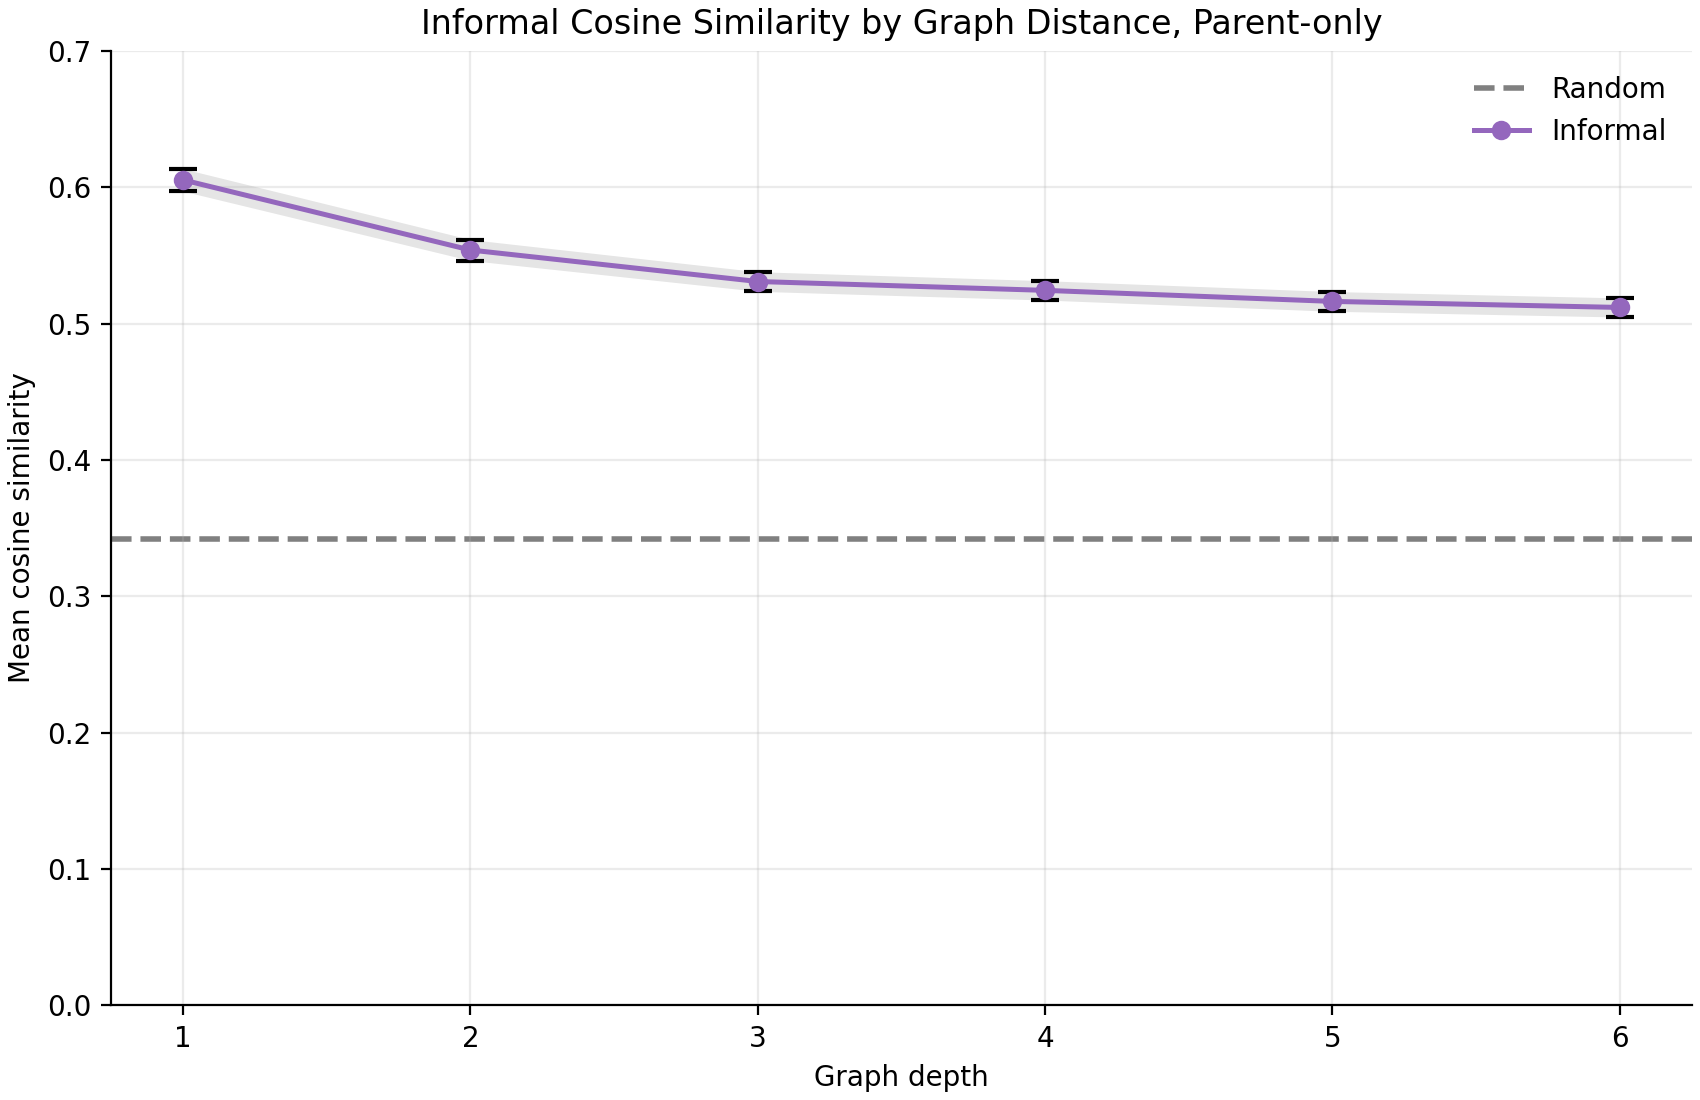
\includegraphics[width=\textwidth]{figures/out/informal-unfixed.png}
        \caption{Informal cosine similarity by $d$-hop distance.}
        \label{fig:graph1}
    \end{subfigure}
    \hfill
    \begin{subfigure}{0.48\textwidth}
        \centering
        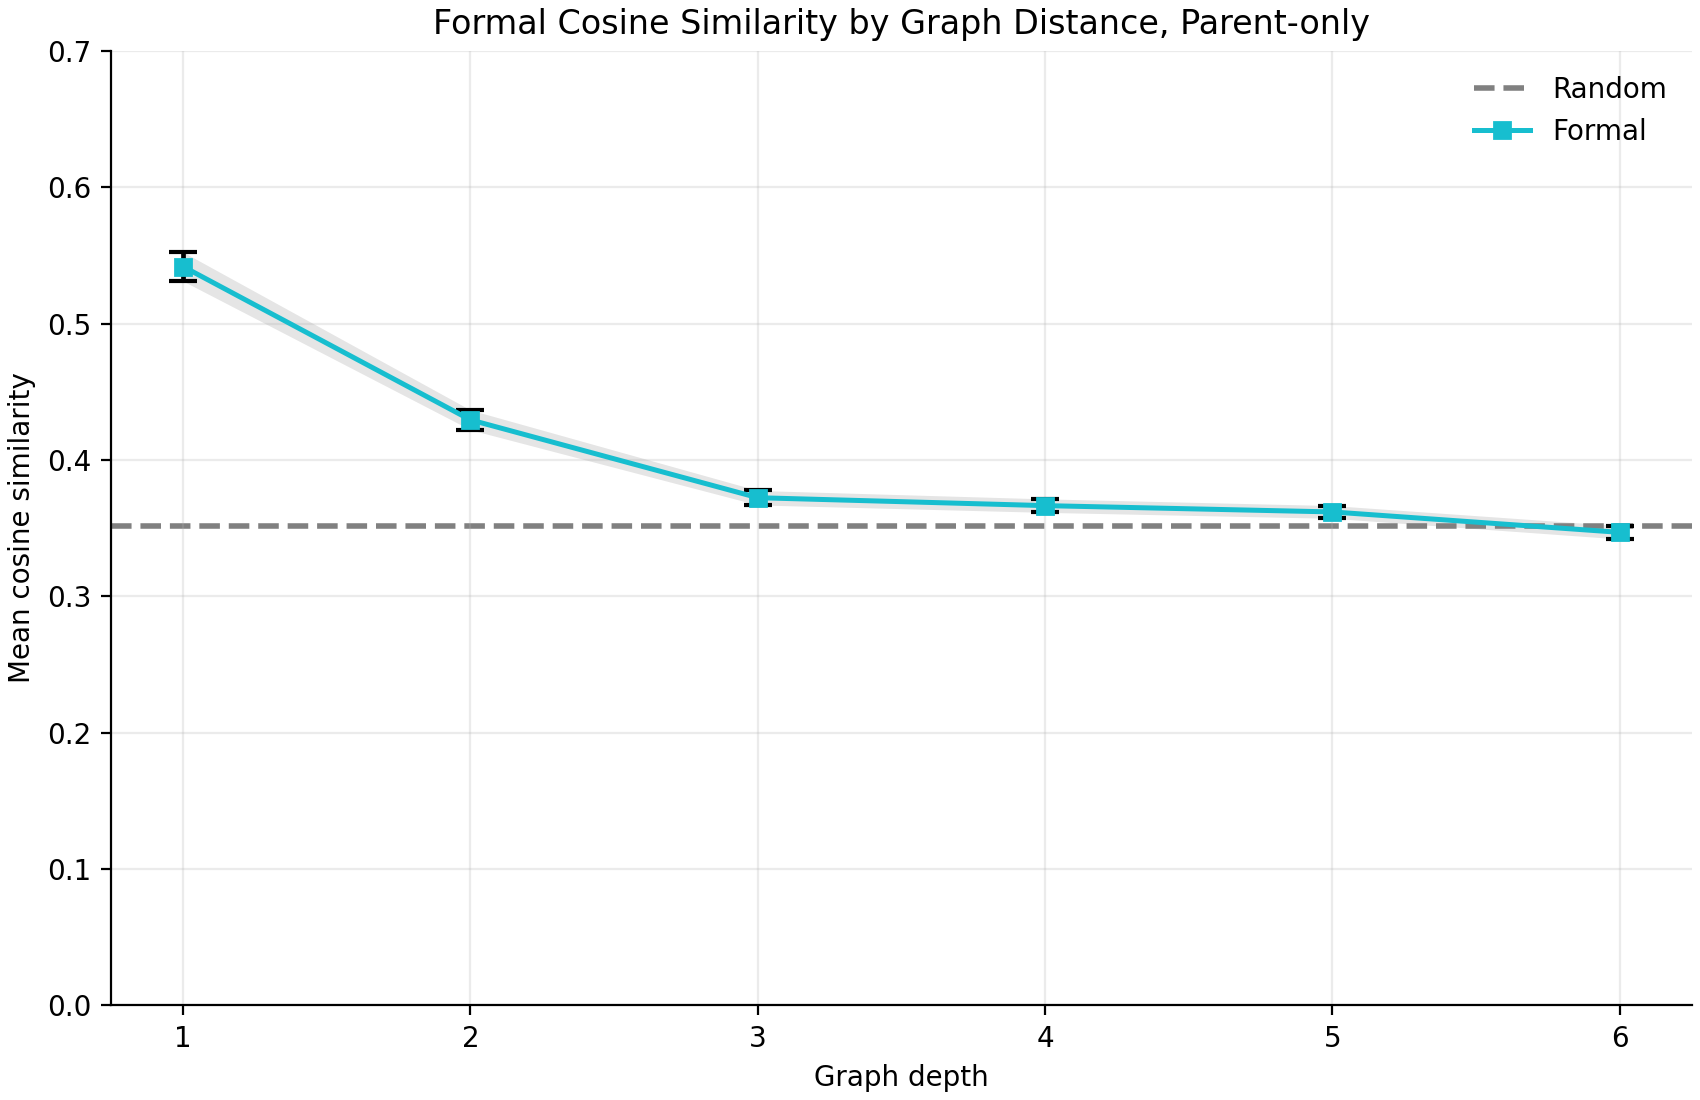
\includegraphics[width=\textwidth]{figures/out/formal-unfixed.png}
        \caption{Formal cosine similarity by $d$-hop distance.}
        \label{fig:graph2}
    \end{subfigure}
    
    \caption{Cosine similarity and node depth for informal and formal graphs.}
    \label{fig:cos-dist}
\end{figure}

Figure~\ref{fig:cos-dist} shows an overall decline in cosine similarity as
directed parent-only graph distance increases in both graphs. The decline is substantially sharper in the formal graph: mean cosine similarity falls from approximately $0.54$ at depth one to roughly the random-pair baseline by depth six. In contrast, informal pairs remain highly similar even at larger graph distances, declining from approximately $0.61$ at depth one to about $0.51$ at depth six, well above the corresponding random baseline.

Thus, under parent-only dependency paths, informal statements retain greater embedding similarity over longer graph distances than formal statements. One possible explanation for the faster decline in the formal graph is its substantially higher local connectivity. Lean records fine-grained dependencies on definitions, typeclass instances, inherited structure, and other reusable mathematical infrastructure. Theorems about a narrow topic may have parent dependencies that connect it to broadly applicable declarations, such as general algebraic or module-theoretic results. Although these edges represent explicit and valid formal dependencies, they need not preserve strong high-level semantic similarity in the generated slogan space. By contrast, informal dependency paths may more often remain within a shared local development or exposition, allowing statements to retain greater embedding similarity over several graph steps.

\subsection{Limitations}

This analysis conditions on successful trajectories whose endpoints have usable slogan embeddings and whose directed shortest-path distance is exactly $d$. As depth increases, obtaining a fixed number of accepted pairs may therefore favor seed statements with sufficiently rich local neighborhoods, longer dependency chains, and reachable embedding-eligible endpoints. The resulting samples may not be representative of all statements at a given graph distance.

Moreover, each depth is sampled independently, and seed statements, nodes, and local neighborhoods may recur across sampled trajectories. The reported pointwise confidence intervals treat observations as independent and therefore may not fully capture uncertainty induced by overlap among walks.